\section{IPI Protocol Design}
\label{sec:ipi}

The preceding literature establishes two requirements for a common application
contract: preserve deployed J2735 messages and represent correlated CAV
operations. IPI implements both requirements through one transport-independent
interface. Stateless CV and ITS exchanges use individual J2735 messages for
vehicle state, signal timing, and intersection geometry. Stateful CAV
operations use requests, updates, and responses that remain associated through
an identity, progress state, and expiration time. Both application classes use
the same vehicles and communication resources. IPI is the first implemented
application protocol that combines the J2735 message set with correlated
stateful CAV operations
~\cite{saej2735_2020,etsi123286r18}.

\textbf{Two interaction modes.}
IPI represents these two application classes through two interaction modes.
Message mode carries individual J2735 messages, including stateless updates,
through typed helpers for Basic
Safety Message (BSM), Personal Safety Message (PSM), Map Data (MAP), Signal
Phase and Timing (SPaT), Signal Request Message (SRM), and Signal Status Message
(SSM). It also preserves pre-encoded J2735 bytes and their declared message
type. Operation mode carries stateful perception, planning, control, or map
operations through registration, heartbeat, request, update, completion,
rejection, telemetry, and termination.

\textbf{Common operation metadata.}
Both interaction modes use a common envelope. The envelope identifies the
message, source, application domain, send time, and selected transport. Session
and correlation identifiers bind responses to an
operation. Requests add vehicle location, capability, horizon, and application
context. Responses add progress, expiration, confidence, and typed or opaque
content. The common metadata identifies individual J2735 messages and
associates CAV responses with one request and deadline.
Figure~\ref{fig:ipi-architecture} shows how both interaction modes pass through
the common IPI envelope before binding to a communication path and transport.

\begin{figure}[t]
  \centering
  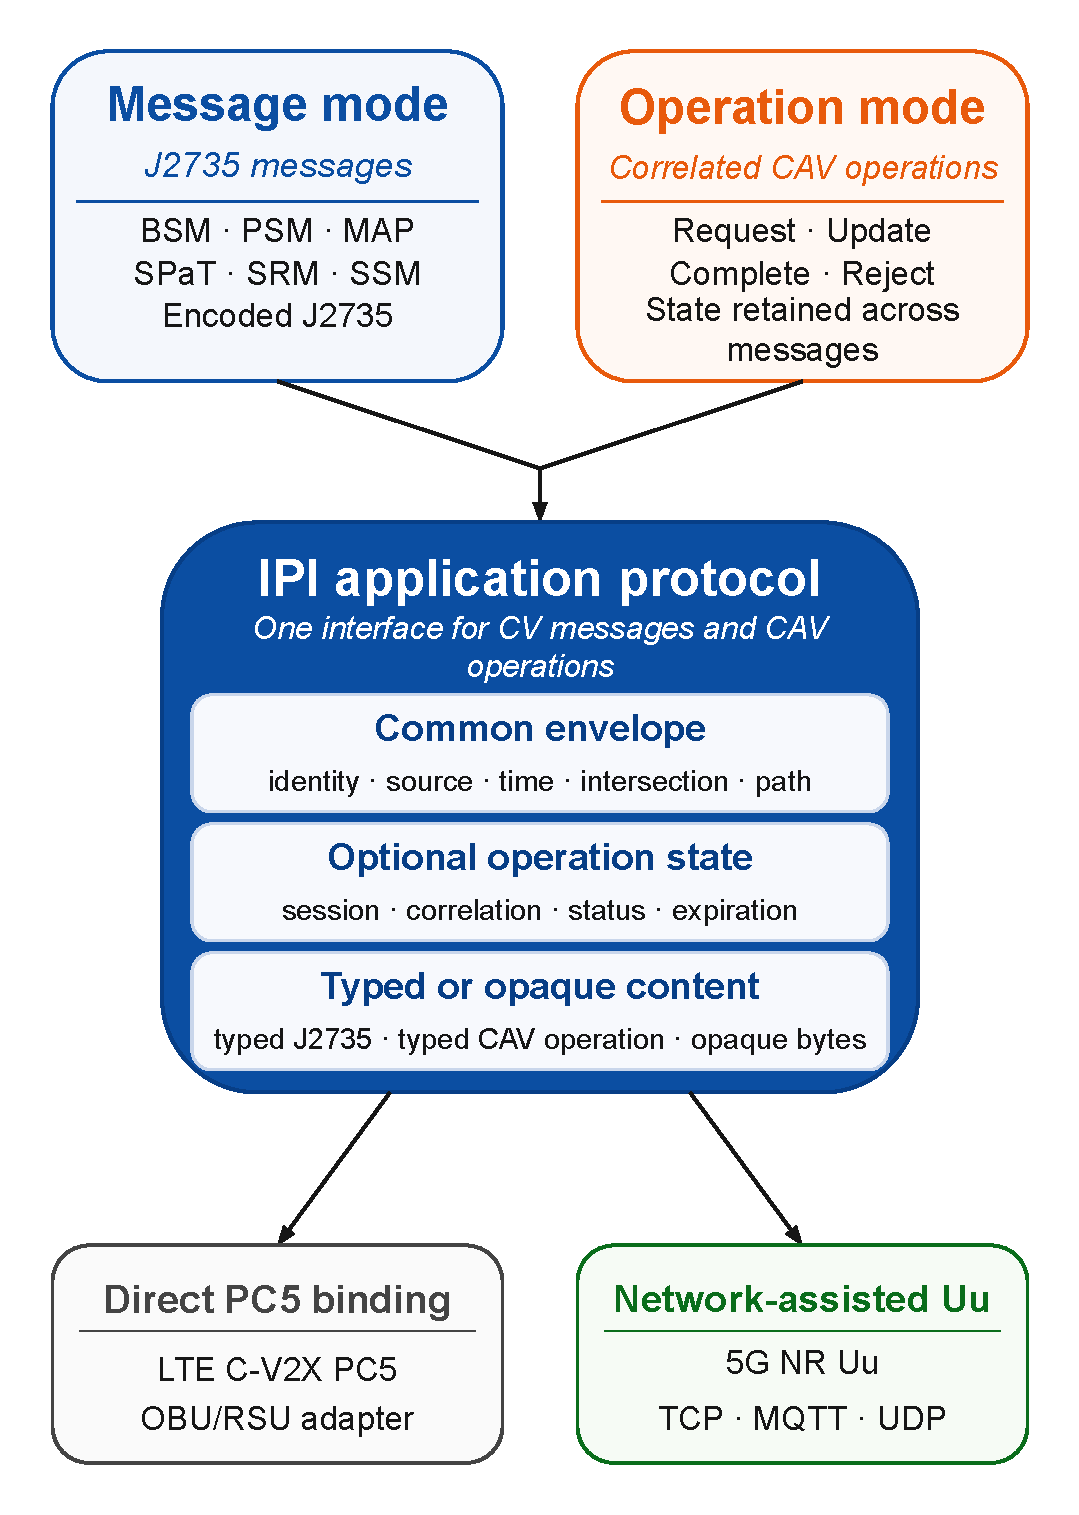
\includegraphics[width=\columnwidth]{../figs/Fig2_ipi_protocol_architecture_editable.pptx.pdf}
  \caption{IPI supports stateless CV/ITS applications and stateful CAV
  applications through one transport-independent application protocol before
  binding their messages and operations to a communication path and transport.}
  \Description{J2735 messages and correlated CAV operations enter the common
  IPI application protocol, which carries envelope metadata, optional operation
  state, and typed or opaque content before binding to direct PC5 or
  network-assisted Uu.}
  \label{fig:ipi-architecture}
\end{figure}

\textbf{Reference implementation and validation.}
The C++17 library implements both modes with message and operation facades,
byte encodings, validators, session records, and communication adapters. Typed helpers map
common J2735 structures into the IPI envelope. The encoded-payload path
preserves the complete J2735 message set. Cooperative requests and responses
use the shared envelope, session, and correlation fields. Seven automated tests cover
typed and pre-encoded messages, cooperative objects, session operations,
malformed input, and Transmission Control Protocol (TCP) and Message Queuing
Telemetry Transport (MQTT) loopback. Section~\ref{sec:results-functional}
quantifies representation overhead for preserved J2735 messages and stateful
CAV operations.
